\documentclass[12pt,fleqn, parskip=full]{scrartcl}

\usepackage{amsmath}
\usepackage{fancyhdr}
\usepackage{graphicx}
\usepackage{float}

\pagestyle{fancy}
\lhead{Donald Doyle UIN: 128005953}

\title{NUEN 301 \\
Homework 2}
\author{Donald Doyle UIN: 128005953}
\date{\today}

\begin{document}

\maketitle

Exercise 1 [30 pts]: [chain reaction] In a certain thermal reactor, for every 100 neutrons emitted in fission, 12 escape while fast, and 3 escape after slowing down to thermal energies. No neutrons are absorbed while slowing down. The values of $\eta_T$ and $\nu_T$ in the fissile material are 2 and 2.5, respectively. The reactor is critical.\\
a. [5 pts]Fill the neutron tree of life, below.
\begin{figure}[H]
	\centering
	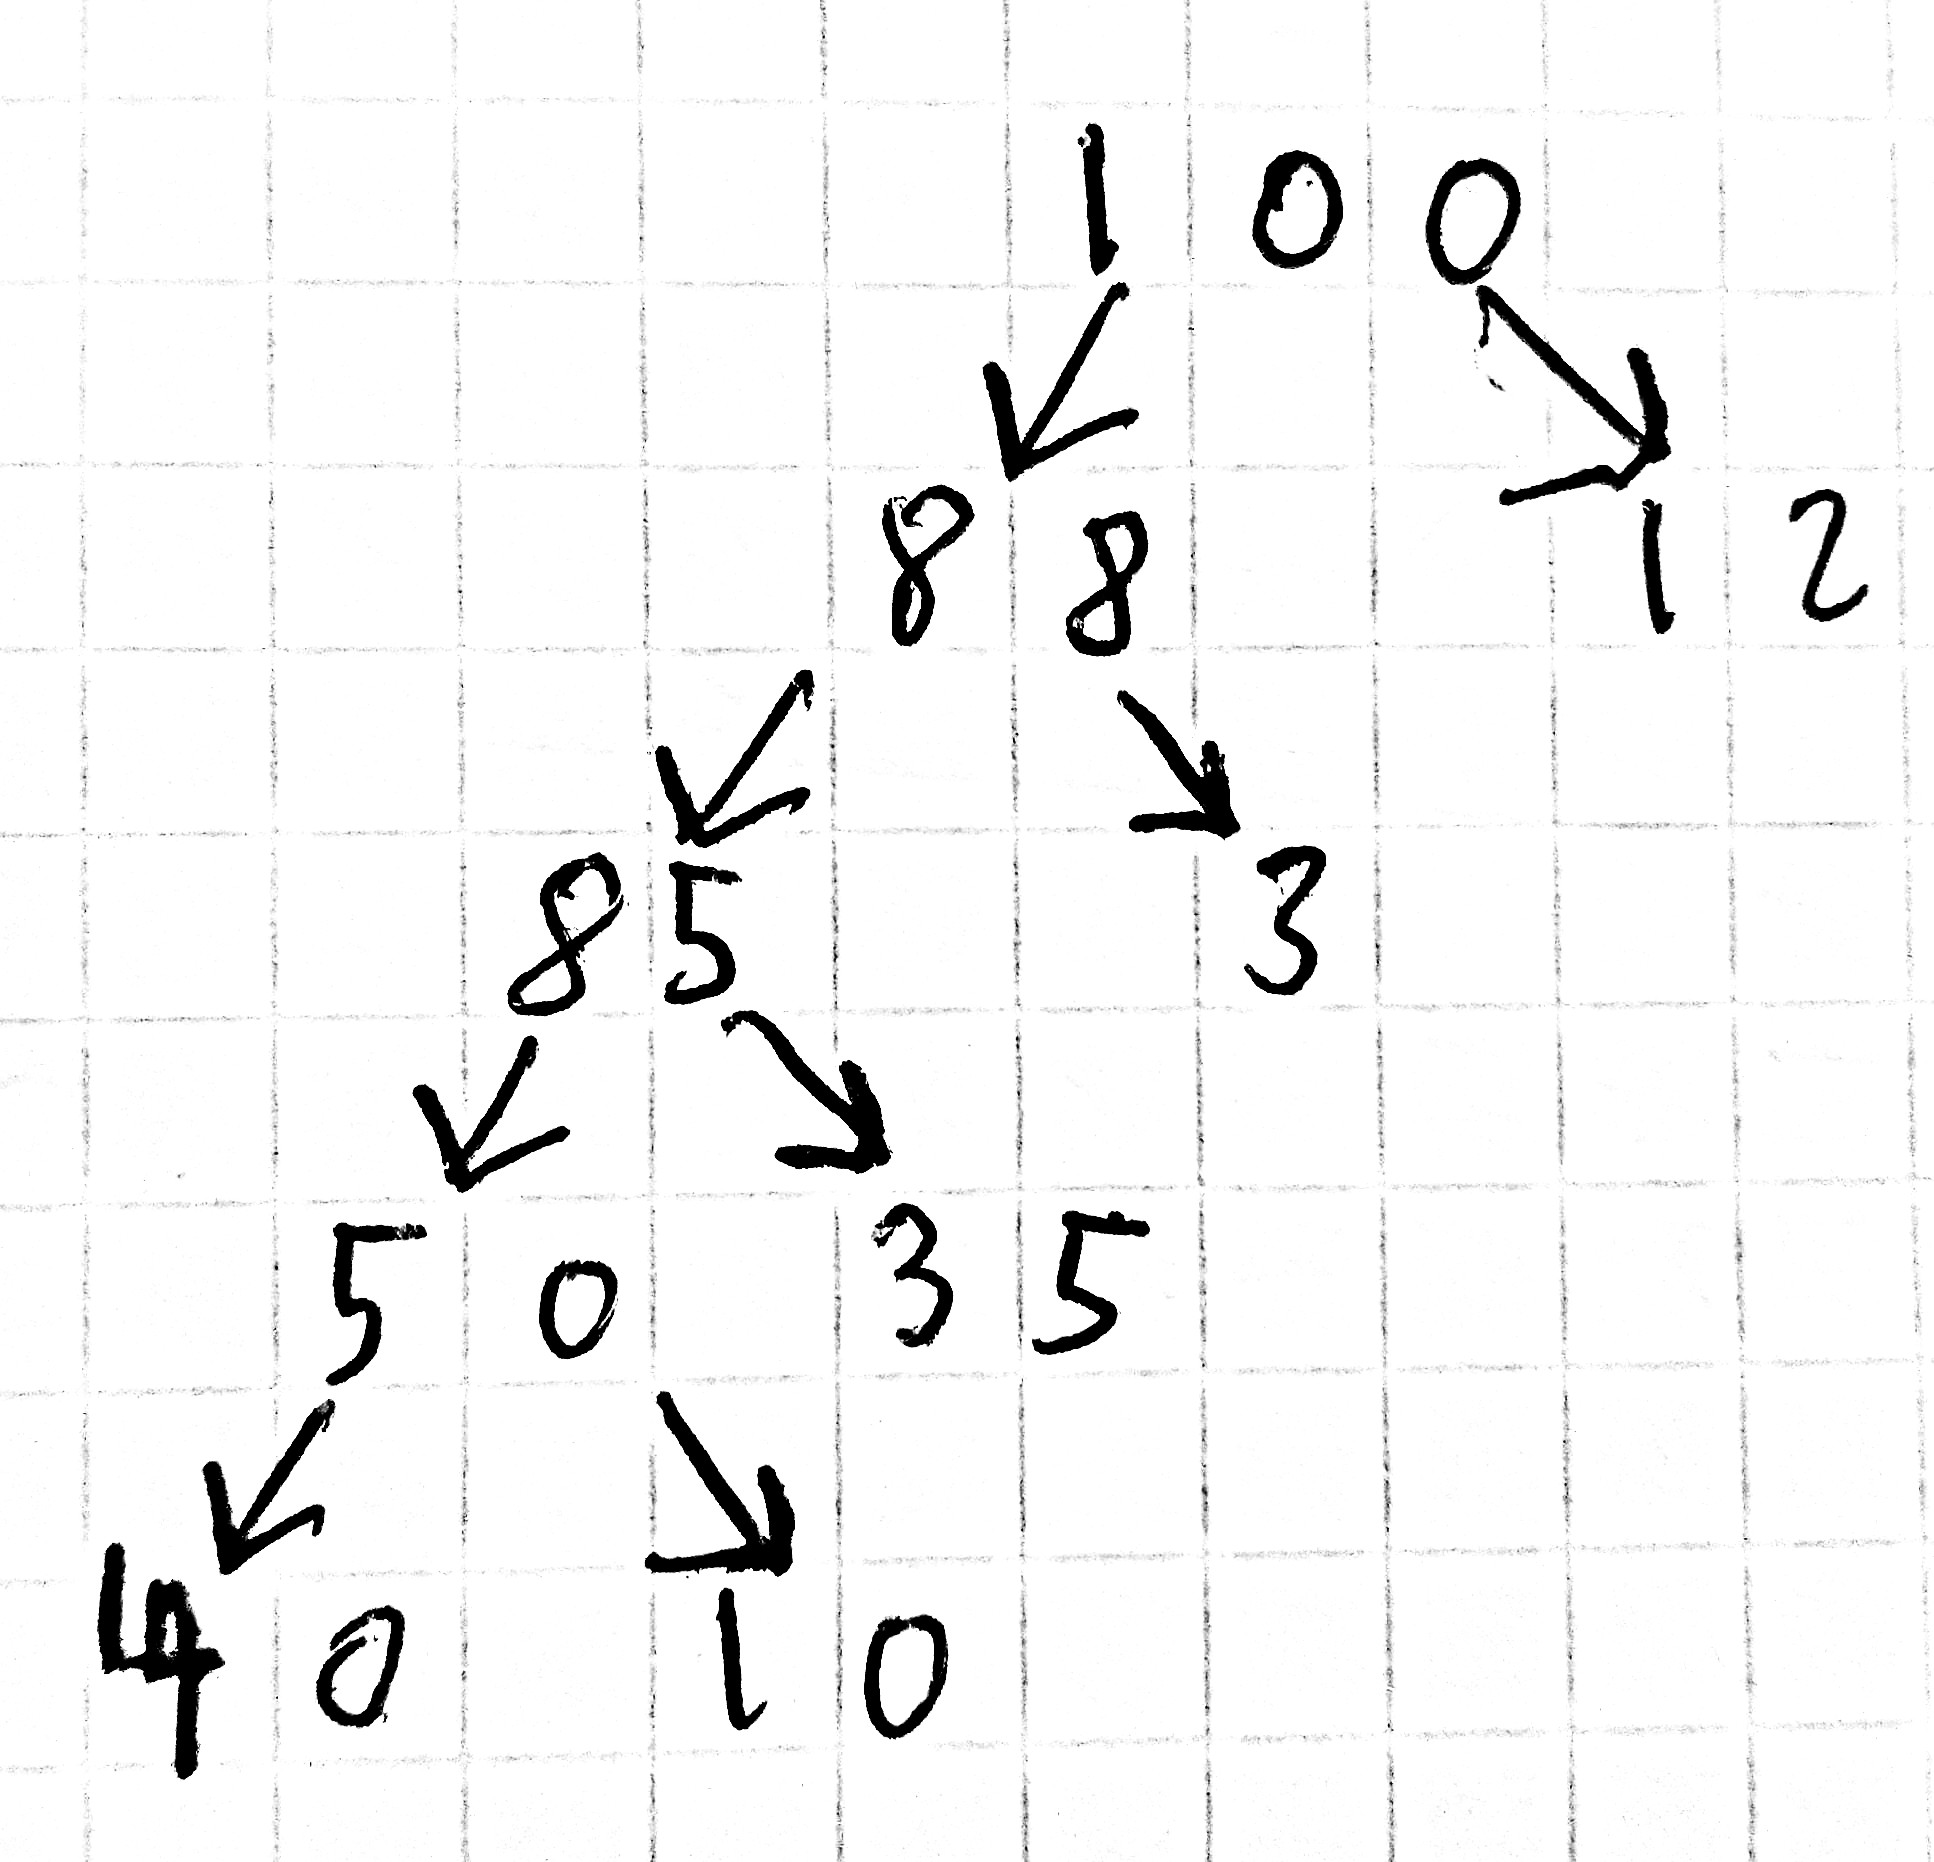
\includegraphics[scale=.1]{Image_1_hw_2}
\end{figure}

b.[5 pts]Calculate the fast non-leakage probability $(P_{FNL})$.\\
$P_{FNL} = \frac{88}{100} = 0.88$\\
c.[5 pts]What is the resonance-escape probability (p)?\\
$p = \frac{88}{88} = 1$\\
d.[5 pts]Calculate the thermal non-leakage probability $(P_{TNL})$. \\
$P_{TNL} = \frac{85}{88} = 0.966$\\
e.[5 pts]Calculate the thermal utilization (f also known as $u_T$). 
$u_T = \frac{50}{85}=0.588$\\
f.[5 pts]Calculate $P_{TAF}$. \\
$P_{TAF} = \frac{\eta_F}{\nu_F} = \frac{2}{2.5} = 0.8$\\

Exercise 2 [30 pts]: [RRD] Ni-63 is a beta- emitter, produced when a thermal neutron is captured in Ni-62 (molar mass 62 g/mol, density 8.9 g/cc). The radiative microscopic cross section of Ni-62 is 15 b when the neutron energy is E=1/40 eV (the cross section has been averaged of the nucleus velocities).  Assume no other types of interactions occur. A thin 0.05-gram target of pure Ni-62 is placed in a beam of thermal neutrons that has intensity $6x10^8$ n/(cm2-s). \\
a.[5 pts]What is the density of the neutrons in the incident beam?\\
$E= \frac{1}{2}mv^2 \Rightarrow v = \sqrt{\frac{2E}{m}} = \sqrt{\frac{2(2.5*10^{-8}[Mev])}{939.6[Mev/c^2]}} = 7.29*10^-4 [cm/s]\\
I=nv \Rightarrow n = \frac{I}{n} = \frac{6x10^8}{7.29*10^-6} = 8.23*10^{11} [n/cm^3]$\\
b.[5 pts]What is the capture rate (captures/second) in the target?\\
$Rate = (15*10^{-24}[\frac{cm^2}{nucleus}])(6*10^8 [n/cm^2-s])(\frac{(8.9)(6.022*10^{23})}{62} [\frac{atoms}{cm^3}])(\frac{8.9}{0.05} [cm^3]) =  1.38*10^{11} [captures/s]$\\
c.[5 pts]At what rate is Ni-63 produced (atoms/second)?\\
1 capture = 1 production so $(8.9)=4.01*10^{-15} [atoms/s]$\\
d.[5 pts]What is the maximum activity that this experiment can produce (the maximum decays of Ni-63 per second)? (Assume that the Ni-63 does not interact with the neutrons, but is lost only via decay.)\\
The maximum decay rate would be equal to the production rate assuming all the Ni-63s decay immediately so $(8.9)=4.01*10^{-15} [decays/s]$\\
e.[10 pts]Suppose another Ni-62 target is now employed. It is thick enough that beam attenuation cannot be neglected. The exit intensity is 25\% lower than the incident bean intensity.\\
i.What is the target thickness?\\
$I=I_0e^{-\Sigma_t x} \Rightarrow x = -\Sigma_t ln(\frac{I}{I_0}) = -(15*10^{-24})(\frac{(8.9)(6.022*10^{23})}{62})ln(\frac{75}{100}) = 0.373 [cm]$ \\
ii.What is the capture rate in this thick target (assume a beam-target interaction area of 3 $cm^2$)?\\
$Rate = (15*10^{-24}[\frac{cm^2}{nucleus}])(6*10^8 [n/cm^2-s])(\frac{(8.9)(6.022*10^{23})}{62} [\frac{atoms}{cm^3}])(3 [cm^2])(0.373 [cm]) =  8.71*10^8 [captures/s]$\\

Exercise 3 [20 pts]: [RRD] The letter T of the A \& M logo is made of texasanmium. Its total cross section for thermal neutrons is 2 cm-1. A beam of thermal neutrons (intensity 105 n/(cm2-s)) is normally incident at x=0. 
\begin{figure}[H]
	\centering
	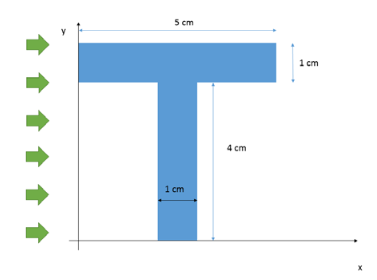
\includegraphics[scale=1]{Image_2_hw_2}
\end{figure}

a.[10 pts]Plot the exiting uncollided intensity as a function of y for x=5cm\\
\begin{figure}[H]
	\centering
	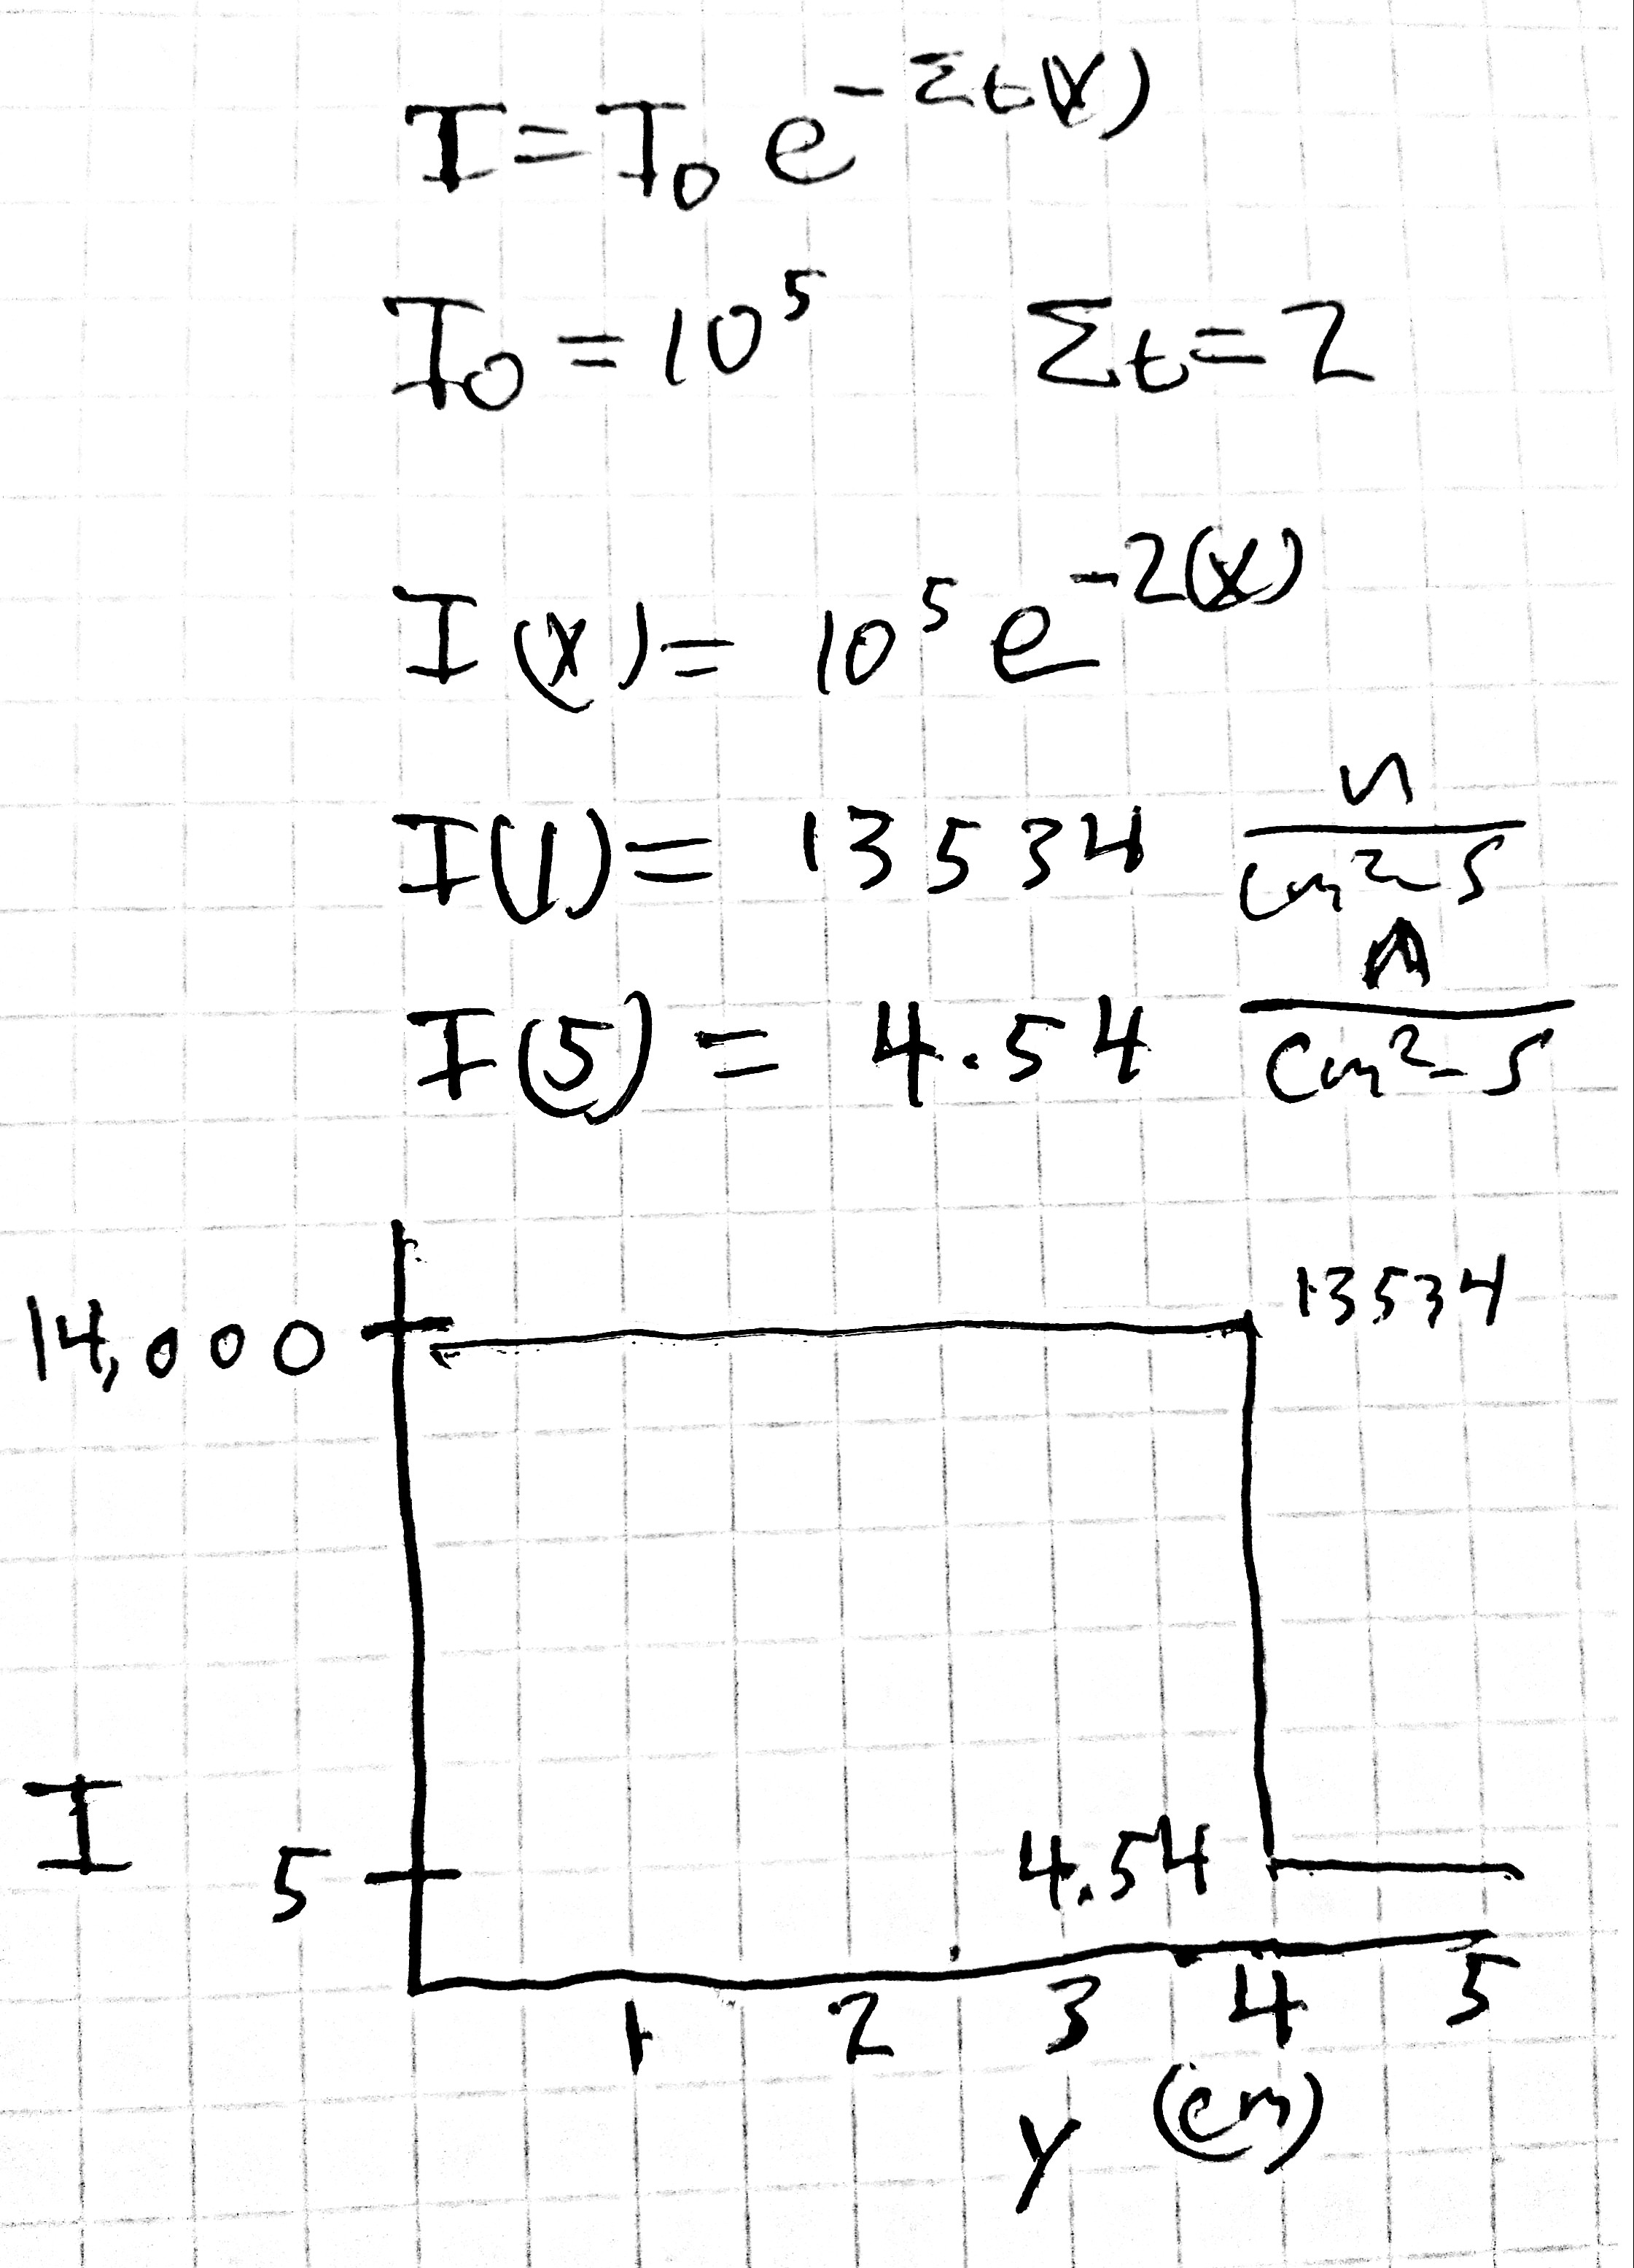
\includegraphics[scale=.1]{Image_3_hw_2}
\end{figure}
b.[10 pts]Assume that the letter T is 1-cm tall along the z-axis and that the beam fully covers the lateral faces, what is the reaction rate (reactions/s) in the letter T.\\
$Rate = (10^5 [\frac{n}{cm^2-s]})(2 [cm^{-1}])((5[cm])(1[cm])+(4[cm])(1[cm]))(1[cm])=1.80*10^6[reactions/s]$\\

Exercise 4 [20 pts]: [Monte Carlo]Reproduce in python the Monte Carlo code shown in class.  Requirements:\\
1. Slab thickness = 20 cm. Macroscopic total XS = 0.2 cm-1. \\
2. Number of bins = 12 \\
a.[5 pts]When running, the code you interactively request the user for the number of neutron histories.\\
b.[5 pts]Provide 3 plots for the flux in the slab using (1) 100 histories, (2) 1,000 histories, (3) 10,000 histories.\\
\begin{figure}[H]
	\centering
	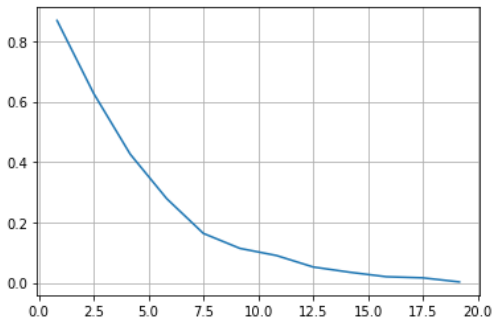
\includegraphics[scale=1]{Image_4_hw_2}
	\caption{100 histories}
\end{figure}
\begin{figure}[H]
	\centering
	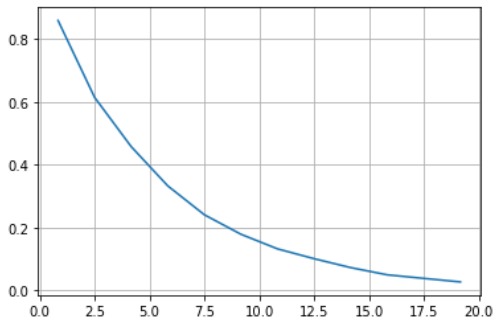
\includegraphics[scale=1]{Image_5_hw_2}
	\caption{1,000 histories}
\end{figure}
\begin{figure}[H]
	\centering
	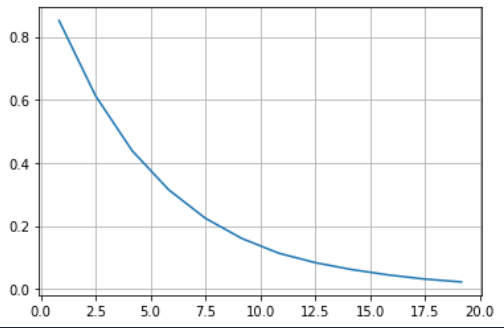
\includegraphics[scale=1]{Image_6_hw_2}
	\caption{10,000 histories}
\end{figure}
c.[5 pts]Provide your code in the HW submission (copy/paste). Code must be clean (meaningful variable names, no superfluous/unused lines of code, adequate comments/documentation)\\
\begin{figure}[H]
	\centering
	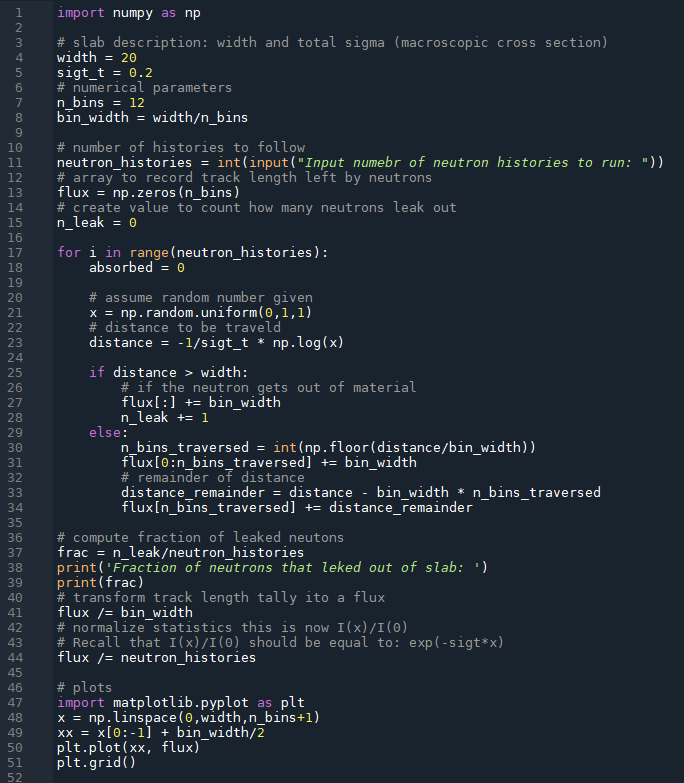
\includegraphics[scale=1]{Image_7_hw_2}
\end{figure}
d.[5 pts]Provide your python code (.py file to be submitted, we will be running the file)\\

Exercise 5 [10 EXTRA pts, MADATORY for Honors]: [Monte Carlo]Compute the fraction of neutrons that leak out of the slab. Provide a table that shows your Monte Carlo code results for 100, 1,000, and 10,000 histories. Compare it against the exact analytical answer.\\
For analytical solution $I=I_0e^{(.2)(20)}$ for the fraction $\frac{I}{I_0}$\\
\begin{table}[H]
\small
\begin{center}
{\begin{tabular}{|c|c|}
\hline
From Code & Analytical\\
\hline
0.0 & 0.018\\
\hline
0.024 & 0.018\\
\hline
0.0193 & 0.018\\
\hline
\end{tabular}}
\end{center}
\end{table}
As expected the Monte Carlo approaches the analytical solution as the number of histories increases.

\end{document}
